\documentclass[english]{article}\usepackage[]{graphicx}\usepackage[]{color}
\usepackage{alltt}
\usepackage[T1]{fontenc}
\usepackage[latin9]{inputenc}
\usepackage{geometry}
\geometry{verbose}
\setcounter{secnumdepth}{2}
\setcounter{tocdepth}{2}
\usepackage{amsmath}
\usepackage{graphicx}
\usepackage{esint}
\usepackage{babel}
\usepackage{verbatim} % for \begin{comment}
\IfFileExists{upquote.sty}{\usepackage{upquote}}{}
\begin{document}

\title{Autonomous Robots and Environmental Mapping}

\author{Mitchell Horning, Matthew Lin, Siddarth Srinivasan, Simon Zou}

\maketitle

\begin{abstract}

Compressed sensing is a technique used to reconstruct sparse signals and images while sampling well below the Nyquist rate. Commonly used in fMRIs and medical imaging, we aim to use this technique to allow autonomous robots to map piecewise constant areas of interest within a larger environment. In our experiment, we programmed a robot equipped with a reflectance sensor to travel along straight-line paths on a black testbed with white regions of interest. The robot integrated sensor readings and sent that sum to a remote server after each path. Each data point consists of the robot's start and end positions, tracked by an overhead camera, and the integral found along that path. Once all the data has been collected, the environment is reconstructed by minimizing the sum of the data fitting term and an L1 penalty term. When using an adaptive path selection scheme, preliminary simulations of our experiment show reconstruction of 100x100 images with only 100 data points (relative err. = 0.28), and we have begun trials with data collected by the robot.

\end{abstract}

\tableofcontents

\section{Introduction}

\begin{comment}
Discuss Compressed Sensing

\end{comment}

Compressed sensing describes a technique in which a signal is reconstructed by 
solving an underdetermined linear system. Doing so allows a signal to be 
found from a relatively small amount of data.

\section{Experiment settings}
\subsection{Testbed}
\subsection{Vehicle hardware}
\subsection{Server}
\begin{comment}
Description of testbed, hardware, software, logic
Sid's flowchart
\end{comment}

\section{Models and assumptions}
\subsection{Constraints}
\begin{comment}
Description of constraints for our problem
limited bandwidth, data storage
Also assumptions about simple piecewise environments
\end{comment}

\section{Algorithm for solving the inverse problem}
\begin{comment}
\end{comment}

\section{Comparison with Other Approaches}
\begin{comment}
\end{comment}
\begin{figure}[h!]
  \centering
    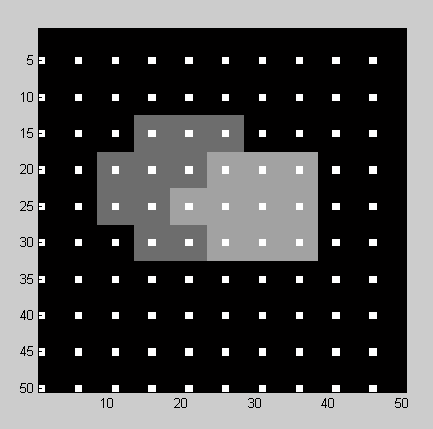
\includegraphics[width=0.5\textwidth]{figures/gridpointexpansion}
  \caption{A picture of a gull.}
  \label{fig:gridpointexpansion}
\end{figure}


\section{Adaptive Pathing}
\begin{comment}
\end{comment}

\section{Conclusions and Further Work}
Figure~\ref{fig:gridpointexpansion} shows a photograph of a gull.

\end{document}
